\section{بحث}

مقادیر RMSE ارائه‌شده در جدول \ref{tab:rmse} و مقایسه‌های تصویری، تفاوت‌های آشکاری در پایداری و دقت روش‌های درون‌یابی نشان می‌دهد. هر چهار روش قادر به بازسازی روند کلی بی‌هنجاری دمای میانگین جهانی در بازه آموزشی هستند، اما عملکرد آن‌ها هنگام تغییر بازه آموزش یا نیاز به برون‌یابی تفاوت چشمگیری پیدا می‌کند.

روش‌های نیوتن پیشرو و پسرو محلی، اگرچه در بازه آموزش داده عملکرد مناسبی دارند، اما نسبت به انتخاب بازه آموزشی بسیار حساس‌اند. با تغییر بازه، مقدار RMSE آن‌ها به شدت افزایش می‌یابد و بررسی نمودارها نشان می‌دهد که انباشتگی خطا (error accumulation) به ویژه در نزدیکی مرزها و خارج از بازه آموزش، مشکل اصلی این روش‌هاست. این پدیده از ویژگی‌های چندجمله‌ای‌های کلاسیک است که خطاهای کوچک در هر گام می‌تواند به سرعت تقویت شده و به ناپایداری و پیش‌بینی‌های غیرقابل اعتماد منجر شود.

درون‌یابی لاگرانژ محلی نیز، هرچند گاهی در نواحی متراکم داده دقت بالایی دارد، اما حتی بیشتر از روش‌های نیوتن دچار انباشتگی خطا و پدیده رانگه می‌شود؛ همان‌طور که RMSE بسیار بزرگ آن در حالت برون‌یابی نشان می‌دهد. این روش به ویژه در برون‌یابی یا داده‌های غیر یکنواخت ناپایدار است.

در مقابل، رگرسیون چندجمله‌ای محلی به عنوان پایدارترین و دقیق‌ترین روش ظاهر می‌شود. مقدار RMSE آن حتی در بازه آموزشی محدود نیز پایین باقی می‌ماند و پیش‌بینی‌هایش کمتر تحت تأثیر انباشتگی خطا قرار می‌گیرد. این روش تعادل مناسبی بین انعطاف‌پذیری و کاهش نویز ایجاد می‌کند و برای درون‌یابی و حتی برون‌یابی محدود داده‌های اقلیمی، انتخاب قابل اعتمادی است.

با توجه به پایداری و تعمیم‌پذیری بالای رگرسیون چندجمله‌ای محلی، از این روش برای پیش‌بینی بی‌هنجاری دمای میانگین جهانی در دهه پیش رو (2020s) استفاده شد. مدل روی بازه کامل [1950, 2020] آموزش داده شد و سپس مقادیر سال‌های 2021 تا 2030 را پیش‌بینی کرد. شکل~\ref{fig:future-prediction} نتایج برون‌یابی را نشان می‌دهد. اگرچه این پیش‌بینی‌ها می‌تواند دید مناسبی نسبت به روندهای احتمالی آینده ارائه دهد، اما باید با احتیاط تفسیر شوند؛ چرا که عدم قطعیت در خارج از بازه داده‌های مشاهده‌شده به سرعت افزایش می‌یابد و رویدادهای غیرمنتظره یا رفتارهای غیرخطی اقلیمی ممکن است توسط مدل پوشش داده نشوند.

\begin{figure}[htbp]
    \centering
    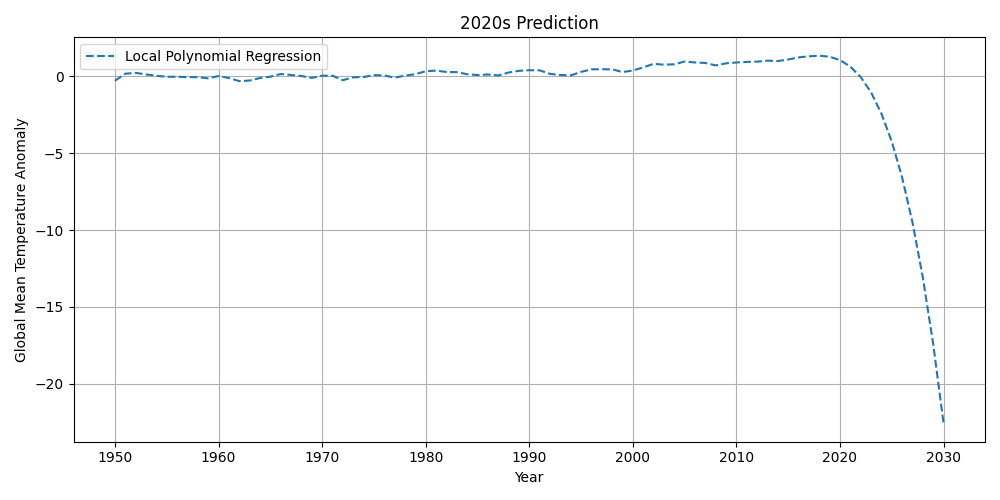
\includegraphics[width=0.8\textwidth]{../figs/2020s-prediction.png}
    \caption{پیش‌بینی رگرسیون چندجمله‌ای محلی برای بی‌هنجاری دمای میانگین جهانی در سال‌های 2021 تا 2030، آموزش‌دیده روی بازه [1950, 2020].}
    \label{fig:future-prediction}
\end{figure}

گام‌های عملی دیگر مانند پاک‌سازی داده‌ها، نرمال‌سازی در پنجره‌های محلی و بازگشت مقاوم به درون‌یابی خطی نیز به افزایش قابلیت اعتماد و تفسیرپذیری نتایج کمک می‌کند.
